\documentclass[sigconf]{acmart}

\usepackage{booktabs} % For formal tables
\usepackage{graphicx}
\usepackage{rotating}
\definecolor{Gray}{gray}{0.6}
\usepackage{tabularx}
\usepackage{xspace}
\usepackage{float}
\usepackage{xstring} % for string operations
\usepackage{wasysym} % Table legend with symbols input from post-processing
\usepackage{MnSymbol} % Table legend with symbols input from post-processing
\usepackage{ifthen}


% Copyright
%\setcopyright{none}
%\setcopyright{acmcopyright}
%\setcopyright{acmlicensed}
\setcopyright{rightsretained}
%\setcopyright{usgov}
%\setcopyright{usgovmixed}
%\setcopyright{cagov}
%\setcopyright{cagovmixed}


% DOI
\acmDOI{10.1145/123_4}

% ISBN
\acmISBN{123-4567-24-567/18/07}

%Conference
\acmConference[GECCO '19]{the Genetic and Evolutionary Computation Conference 2019}{July 13--17, 2019}{Prague, Czech Republic}
\acmYear{2019}
\copyrightyear{2019}

\acmPrice{15.00}



%%%%%%%%%%%%%%%%%%%%%%   END OF PREAMBLE   %%%%%%%%%%%%%%%%%%%%%%%%%%%%%%%%%%%%

%%%%%%%%%%%%%%%%%%%%%%%%%%%%%%%%%%%%%%%%%%%%%%%%%%%%%%%%%%%%%%%%%%%%%%%%%%%%%%%
%%%%%%%%% TO BE EDITED %%%%%%%%%%%%%%%%%%%%%%%%%%%%%%%%%%%%%%%%%%%%%%%%%%%%%%%%
%%%%%%%%%%%%%%%%%%%%%%%%%%%%%%%%%%%%%%%%%%%%%%%%%%%%%%%%%%%%%%%%%%%%%%%%%%%%%%%

% Algorithm names as they appear in the tables, uncomment and adapt if necessary
% \newcommand{\algAtables}{ALGO1}  % first argument in the post-processing
% \newcommand{\algBtables}{ALGO2}  % second argument in the post-processing
% \newcommand{\algCtables}{ALGO3}  % third argument in the post-processing
% \newcommand{\algDtables}{ALGO4}  % fourth argument in the post-processing
% ...
% location of pictures files
\newcommand{\bbobdatapath}{ppdata/} % change default output folder of COCO if desired
\input{\bbobdatapath cocopp_commands.tex}
\graphicspath{{\bbobdatapath\algsfolder}}

%%%%%%%%%%%%%%%%%%%%%%%%%%%%%%%%%%%%%%%%%%%%%%%%%%%%%%%%%%%%%%%%%%%%%%%%%%%%%%%
%%%%%%%%%%%%%%%%%%%%%%%%%%%%%%%%%%%%%%%%%%%%%%%%%%%%%%%%%%%%%%%%%%%%%%%%%%%%%%%
%%%%%%%%%%%%%%%%%%%%%%%%%%%%%%%%%%%%%%%%%%%%%%%%%%%%%%%%%%%%%%%%%%%%%%%%%%%%%%%

\newcommand{\DIM}{\ensuremath{\mathrm{DIM}}}
\newcommand{\ERT}{\ensuremath{\mathrm{ERT}}}
\newcommand{\FEvals}{\ensuremath{\mathrm{FEvals}}}
\newcommand{\nruns}{\ensuremath{\mathrm{Nruns}}}
\newcommand{\Dfb}{\ensuremath{\Delta f_{\mathrm{best}}}}
\newcommand{\Df}{\ensuremath{\Delta f}}
\newcommand{\DI}{\ensuremath{\Delta I_{\mathrm{HV}}^{\mathrm{COCO}}}}
\newcommand{\nbFEs}{\ensuremath{\mathrm{\#FEs}}}
\newcommand{\ftarget}{\ensuremath{f_\mathrm{t}}}
\newcommand{\Itarget}{\ensuremath{I_\mathrm{target}}}
\newcommand{\CrE}{\ensuremath{\mathrm{CrE}}}
\newcommand{\hvref}{\ensuremath{I_\mathrm{ref}}}
\newcommand{\fopt}{\hvref}
\newcommand{\change}[1]{{\color{red} #1}}
\newcommand{\TODO}[1]{{\color{orange} !!! #1 !!!}}
\newcommand{\bbobbiobj}{{\ttfamily bbob-biobj}\xspace}


%%%%%%%%%%%%%%%%%%%%%%   END OF PREAMBLE   %%%%%%%%%%%%%%%%%%%%%%%%%%%%%%%%%%%%

\begin{document}


\title{Black-Box Optimization Benchmarking Template for the Comparison of Multiple Algorithms on the Biobjective \bbobbiobj Testbed}
\renewcommand{\shorttitle}{Template to Compare Multiple Algorithms on the \bbobbiobj Testbed}
\titlenote{Submission deadline: April 3rd.}
%Camera-ready paper due April 24th.}}
\subtitle{Draft version}



\author{Firstname Lastname}
%\authornote{tba if needed}
%\orcid{1234-5678-9012}
%\affiliation{%
%  \institution{Institute for Clarity in Documentation}
%  \streetaddress{P.O. Box 1212}
%  \city{Dublin} 
%  \state{Ohio} 
%  \postcode{43017-6221}
%}
%\email{trovato@corporation.com}
%
%\author{G.K.M. Tobin}
%\authornote{The secretary disavows any knowledge of this author's actions.}
%\affiliation{%
%  \institution{Institute for Clarity in Documentation}
%  \streetaddress{P.O. Box 1212}
%  \city{Dublin} 
%  \state{Ohio} 
%  \postcode{43017-6221}
%}
%\email{webmaster@marysville-ohio.com}
%
%\author{Lars Th{\o}rv{\"a}ld}
%\authornote{This author is the
%  one who did all the really hard work.}
%\affiliation{%
%  \institution{The Th{\o}rv{\"a}ld Group}
%  \streetaddress{1 Th{\o}rv{\"a}ld Circle}
%  \city{Hekla} 
%  \country{Iceland}}
%\email{larst@affiliation.org}
%
%\author{Lawrence P. Leipuner}
%\affiliation{
%  \institution{Brookhaven Laboratories}
%  \streetaddress{P.O. Box 5000}}
%\email{lleipuner@researchlabs.org}
%
%\author{Sean Fogarty}
%\affiliation{%
%  \institution{NASA Ames Research Center}
%  \city{Moffett Field}
%  \state{California} 
%  \postcode{94035}}
%\email{fogartys@amesres.org}
%
%\author{Charles Palmer}
%\affiliation{%
%  \institution{Palmer Research Laboratories}
%  \streetaddress{8600 Datapoint Drive}
%  \city{San Antonio}
%  \state{Texas} 
%  \postcode{78229}}
%\email{cpalmer@prl.com}
%
%\author{John Smith}
%\affiliation{\institution{The Th{\o}rv{\"a}ld Group}}
%\email{jsmith@affiliation.org}
%
%\author{Julius P.~Kumquat}
%\affiliation{\institution{The Kumquat Consortium}}
%\email{jpkumquat@consortium.net}

% The default list of authors is too long for headers}
\renewcommand{\shortauthors}{Firstname Lastname et. al.}


\begin{abstract}
to be written
\end{abstract}


%
% The code below should be generated by the tool at
% http://dl.acm.org/ccs.cfm
% Please copy and paste the code instead of the example below. 
%
 \begin{CCSXML}
<ccs2012>
<concept>
<concept_id>10010147.10010178.10010205.10010208</concept_id>
<concept_desc>Computing methodologies~Continuous space search</concept_desc>
<concept_significance>500</concept_significance>
</concept>
</ccs2012>
\end{CCSXML}

\ccsdesc[500]{Computing methodologies~Continuous space search}


% We no longer use \terms command
%\terms{Algorithms}

% Complete with anything that is needed
\keywords{Benchmarking, Black-box optimization, Bi-objective optimization}

\maketitle


% \section{Introduction}
%
% \section{Algorithm Presentation}
%
% \section{Experimental Procedure}
%

%%%%%%%%%%%%%%%%%%%%%%%%%%%%%%%%%%%%%%%%%%%%%%%%%%%%%%%%%%%%%%%%%%%%%%%%%%%%%%%
\section{CPU Timing}
%%%%%%%%%%%%%%%%%%%%%%%%%%%%%%%%%%%%%%%%%%%%%%%%%%%%%%%%%%%%%%%%%%%%%%%%%%%%%%%
% note that the following text is just a proposal and can/should be changed to your needs:
In order to evaluate the CPU timing of the algorithm, we have run the \change{\algorithmA} with restarts on the entire bbob-biobj test suite \cite{biobj2016func} for $2 D$ function evaluations according to \cite{hansen2016exp}. The \change{C/Java/Matlab/Octave/Python} code was run on a \change{Mac Intel(R) Core(TM) i5-2400S CPU @ 2.50GHz} with \change{1} processor and \change{4} cores \change{and (compile) options xxx}. The time per function evaluation for dimensions 2, 3, 5, 10, 20\change{, 40} equals \change{$x.x$}, \change{$x.x$}, \change{$x.x$}, \change{$xx$}, \change{$xxx$}\change{, and $xxx$} seconds respectively. 

\change{repeat the above for any algorithm tested}

%%%%%%%%%%%%%%%%%%%%%%%%%%%%%%%%%%%%%%%%%%%%%%%%%%%%%%%%%%%%%%%%%%%%%%%%%%%%%%%
\section{Results}
%%%%%%%%%%%%%%%%%%%%%%%%%%%%%%%%%%%%%%%%%%%%%%%%%%%%%%%%%%%%%%%%%%%%%%%%%%%%%%%

Results from experiments according to \cite{hansen2016exp},
\cite{hansen2016perfass} and \cite{biobj2016perfass} on the benchmark
functions given in \cite{biobj2016func} are presented in
Figures~\ref{fig:ECDFsingleOne}, \ref{fig:ECDFsingleTwo}, \ref{fig:ECDFsGroupsFive} and
\ref{fig:ECDFsGroupsTwenty} and in Tables~\ref{tab:ERTs5} and~\ref{tab:ERTs20}.
The experiments were performed with COCO \cite{hansen2020cocoplat}, version
\change{2.4}, the plots were produced with version \change{2.4}.

The \textbf{expected runtime (ERT)}, used in the %figures and
tables,
depends on a given quality indicator value, $\Itarget=\hvref+\DI$, and is
computed over all relevant trials as the number of function
evaluations executed during each trial while the best indicator value
did not reach \Itarget, summed over all trials and divided by the
number of trials that actually reached \Itarget\
\cite{hansen2016exp,price1997dev}.  \textbf{Statistical significance}
is tested with the rank-sum test for a given target $\Itarget$
using, for each trial,
either the number of needed function evaluations to reach
$\Itarget$ (inverted and multiplied by $-1$), or, if the target
was not reached, the best $\DI$-value achieved, measured only up to
the smallest number of overall function evaluations for any
unsuccessful trial under consideration.



%%%%%%%%%%%%%%%%%%%%%%%%%%%%%%%%%%%%%%%%%%%%%%%%%%%%%%%%%%%%%%%%%%%%%%%%%%%%%%%
%%%%%%%%%%%%%%%%%%%%%%%%%%%%%%%%%%%%%%%%%%%%%%%%%%%%%%%%%%%%%%%%%%%%%%%%%%%%%%%

% ECDFs per function in dimension 10

%%%%%%%%%%%%%%%%%%%%%%%%%%%%%%%%%%%%%%%%%%%%%%%%%%%%%%%%%%%%%%%%%%%%%%%%%%%%%%%
\begin{figure*}
\centering
\begin{tabular}{@{\hspace*{-0.00\textwidth}}l@{\hspace*{-0.00\textwidth}}l@{\hspace*{-0.00\textwidth}}l@{\hspace*{-0.00\textwidth}}l@{\hspace*{-0.00\textwidth}}l@{\hspace*{-0.00\textwidth}}}
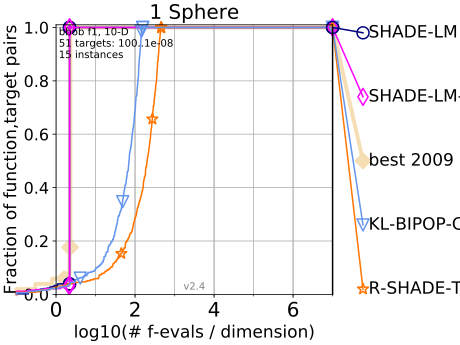
\includegraphics[width=0.2\textwidth]{pprldmany-single-functions/pprldmany_f001_10D}&
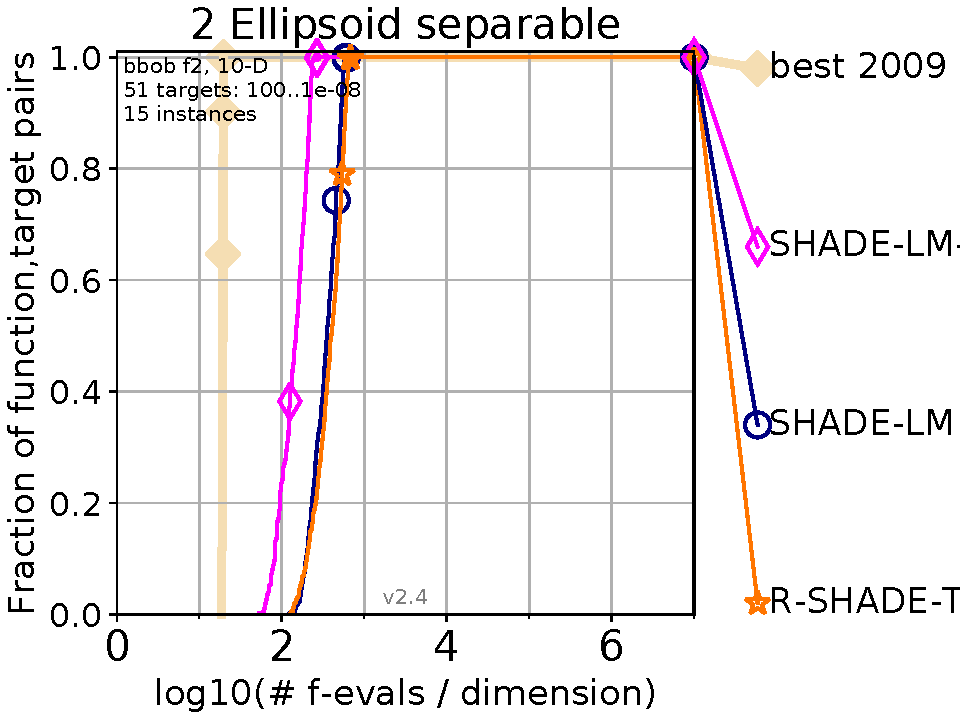
\includegraphics[width=0.2\textwidth]{pprldmany-single-functions/pprldmany_f002_10D}&
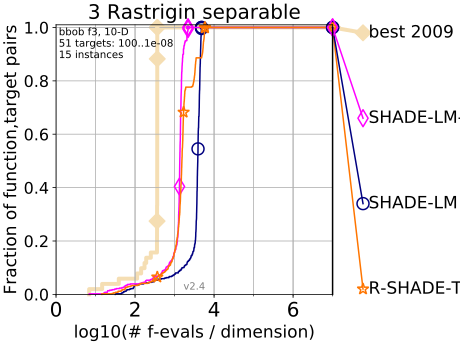
\includegraphics[width=0.2\textwidth]{pprldmany-single-functions/pprldmany_f003_10D}&
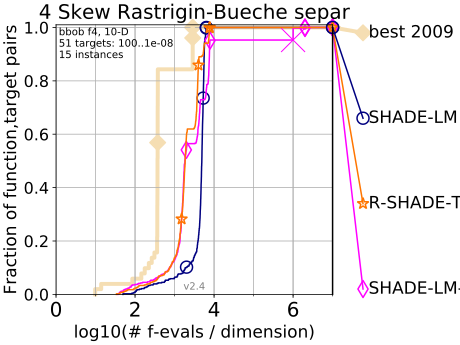
\includegraphics[width=0.2\textwidth]{pprldmany-single-functions/pprldmany_f004_10D}&
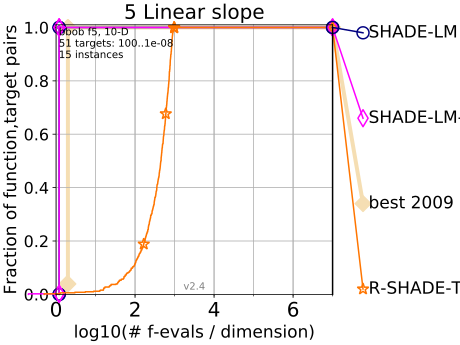
\includegraphics[width=0.2\textwidth]{pprldmany-single-functions/pprldmany_f005_10D}\\
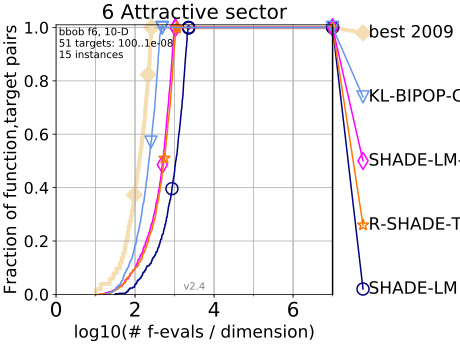
\includegraphics[width=0.2\textwidth]{pprldmany-single-functions/pprldmany_f006_10D}&
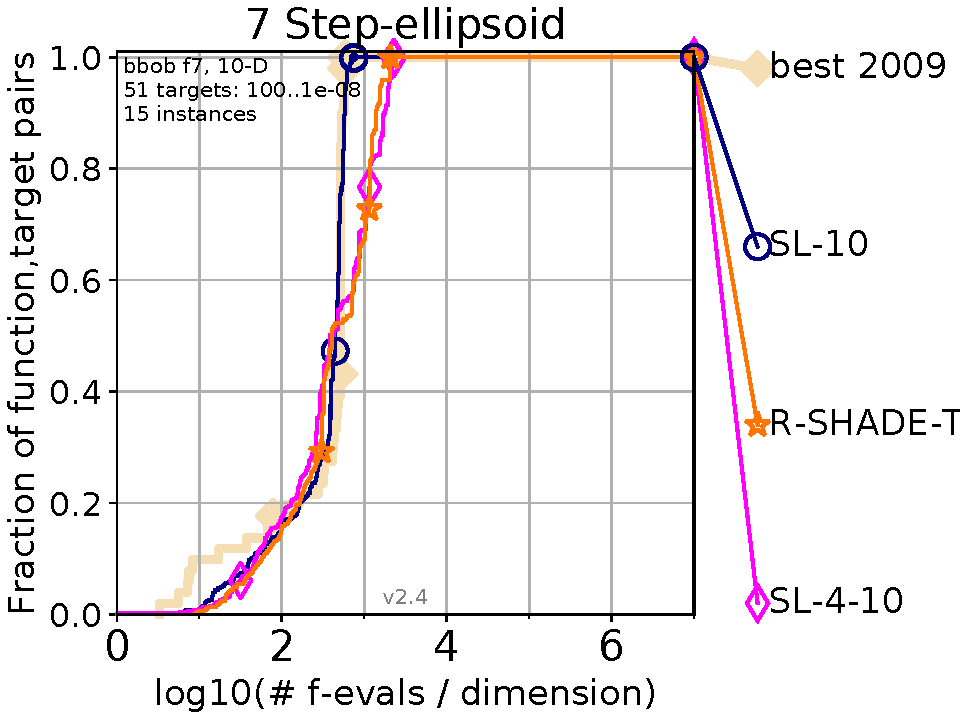
\includegraphics[width=0.2\textwidth]{pprldmany-single-functions/pprldmany_f007_10D}&
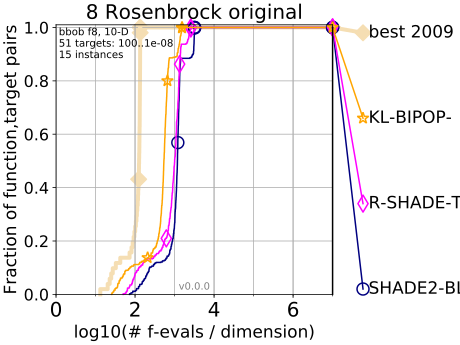
\includegraphics[width=0.2\textwidth]{pprldmany-single-functions/pprldmany_f008_10D}&
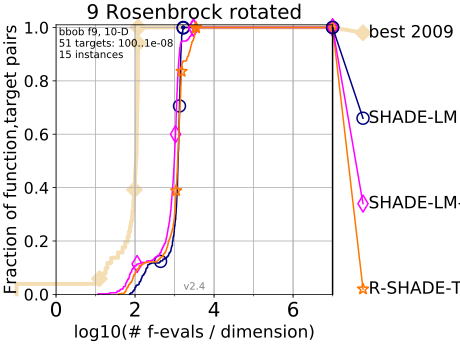
\includegraphics[width=0.2\textwidth]{pprldmany-single-functions/pprldmany_f009_10D}&
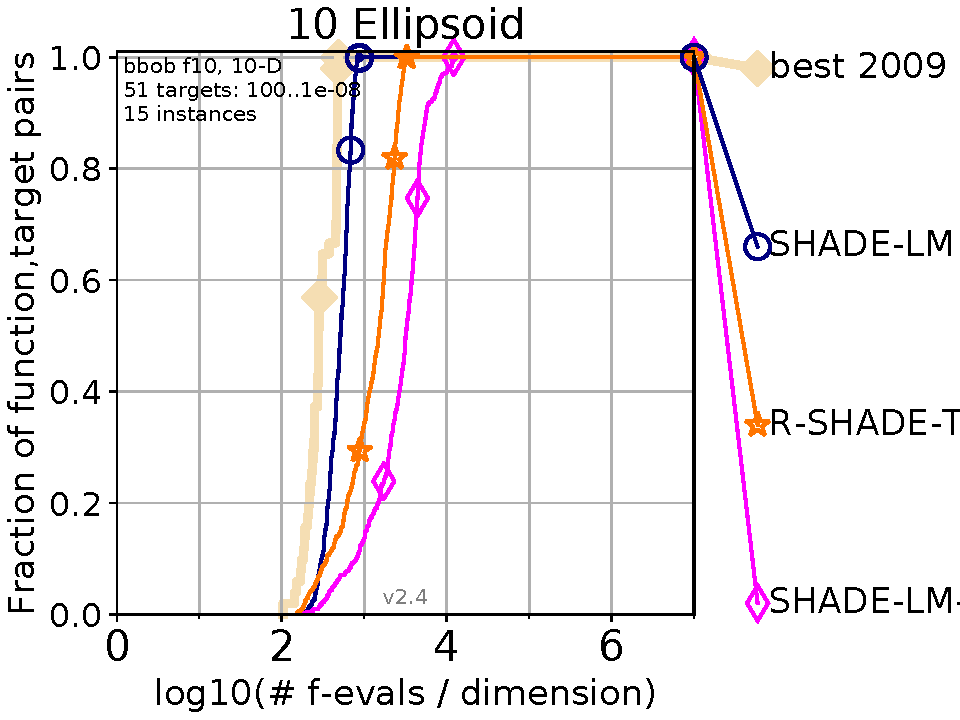
\includegraphics[width=0.2\textwidth]{pprldmany-single-functions/pprldmany_f010_10D}\\
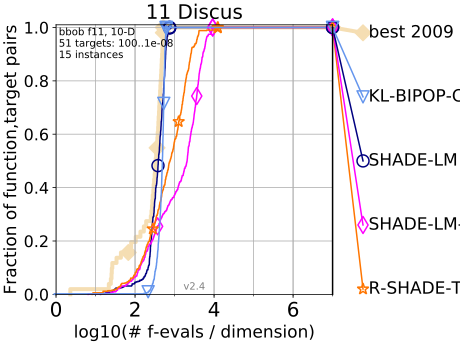
\includegraphics[width=0.2\textwidth]{pprldmany-single-functions/pprldmany_f011_10D}&
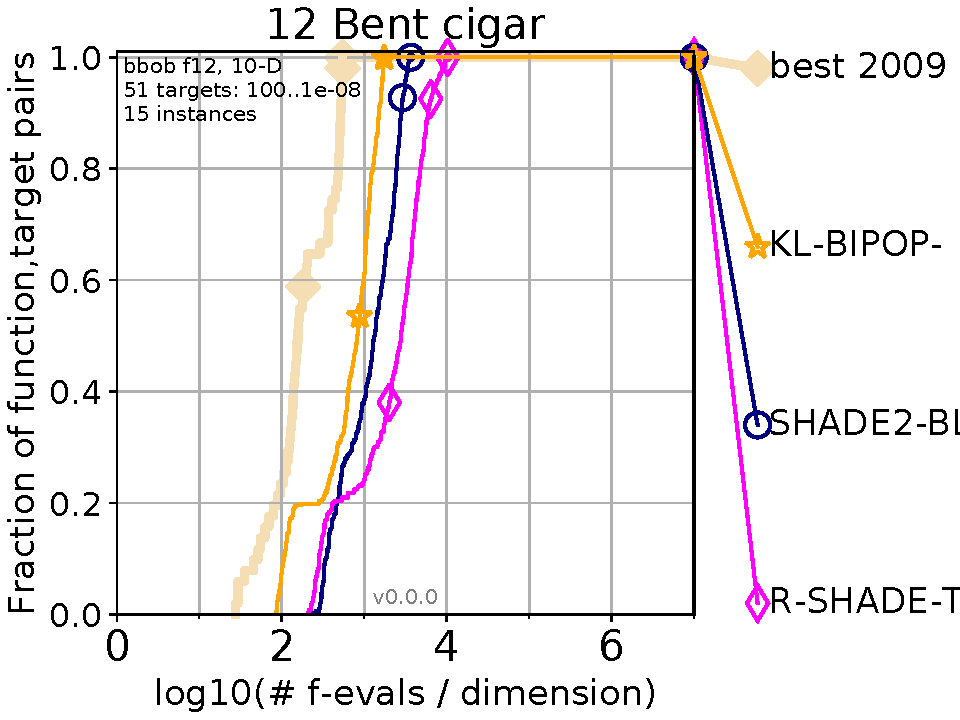
\includegraphics[width=0.2\textwidth]{pprldmany-single-functions/pprldmany_f012_10D}&
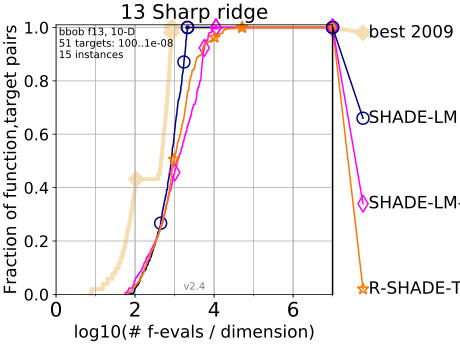
\includegraphics[width=0.2\textwidth]{pprldmany-single-functions/pprldmany_f013_10D}&
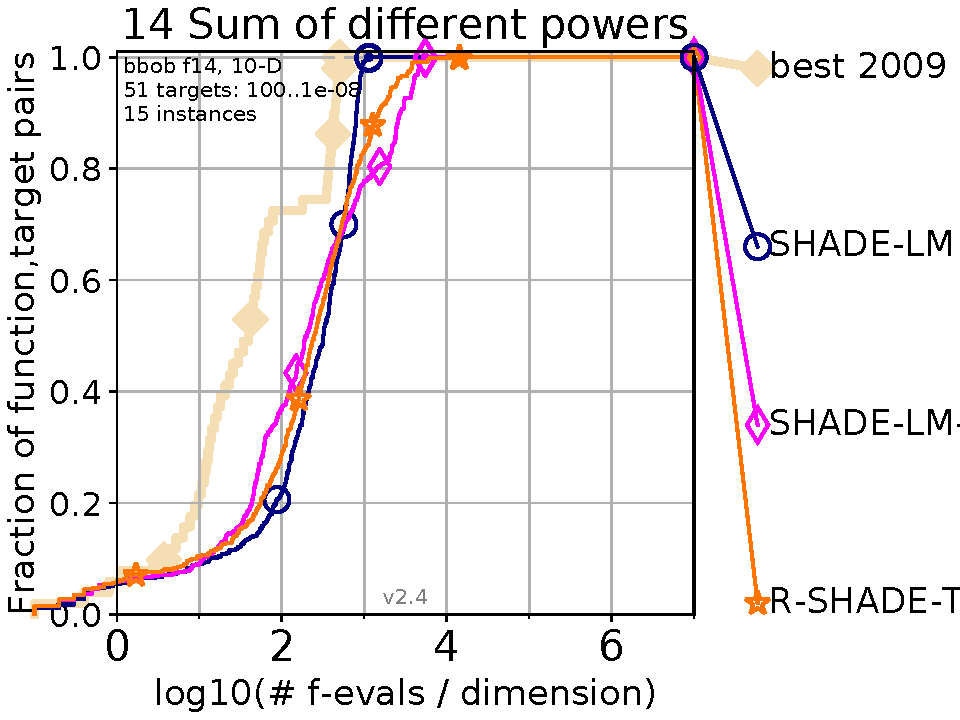
\includegraphics[width=0.2\textwidth]{pprldmany-single-functions/pprldmany_f014_10D}&
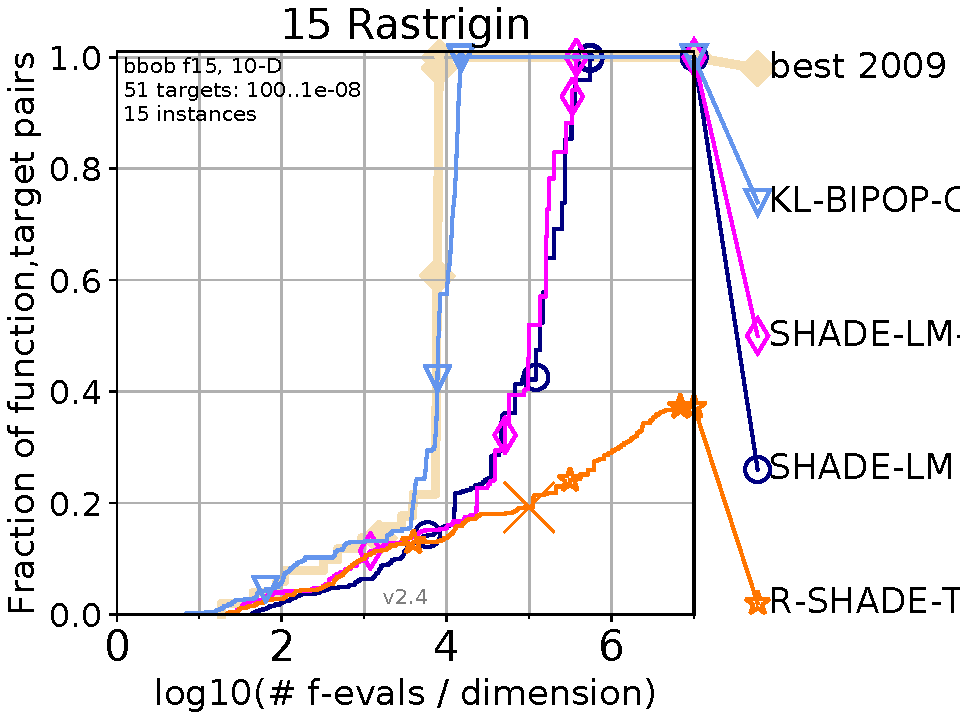
\includegraphics[width=0.2\textwidth]{pprldmany-single-functions/pprldmany_f015_10D}\\
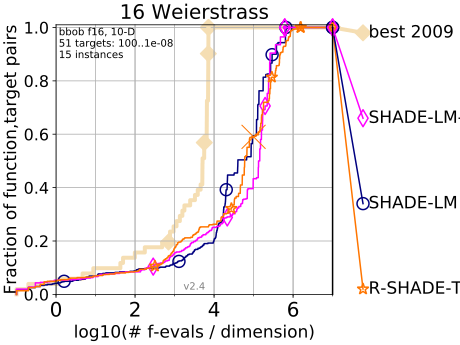
\includegraphics[width=0.2\textwidth]{pprldmany-single-functions/pprldmany_f016_10D}&
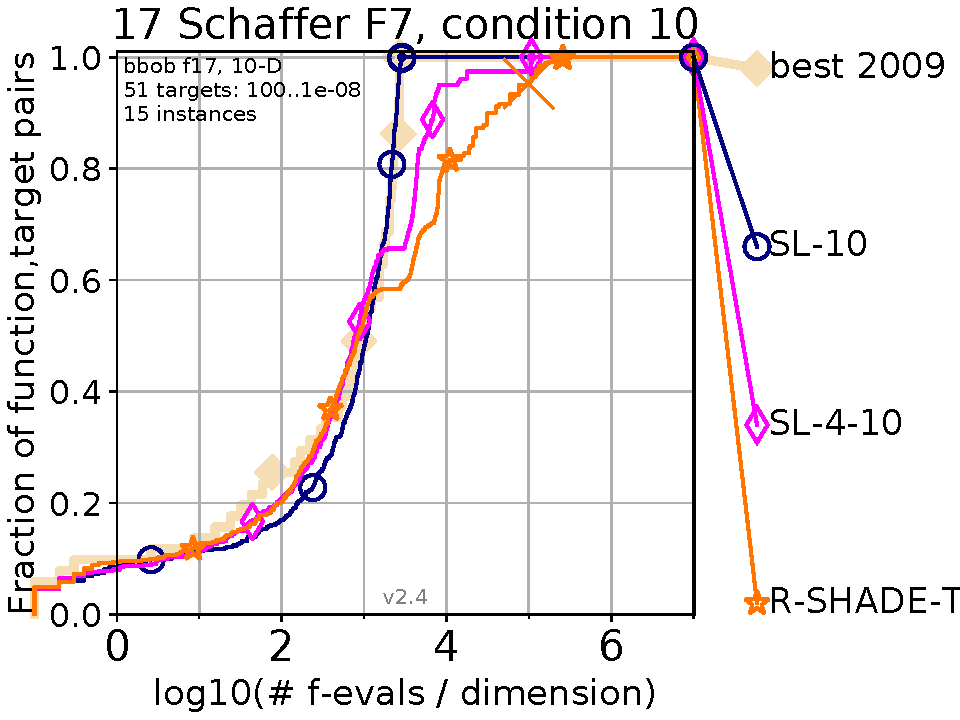
\includegraphics[width=0.2\textwidth]{pprldmany-single-functions/pprldmany_f017_10D}&
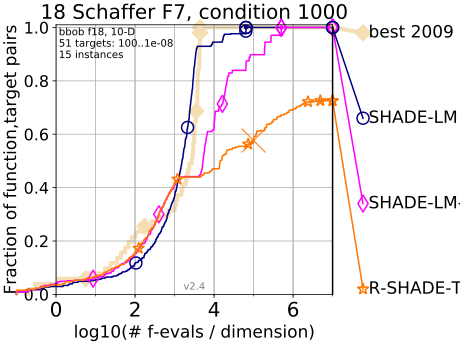
\includegraphics[width=0.2\textwidth]{pprldmany-single-functions/pprldmany_f018_10D}&
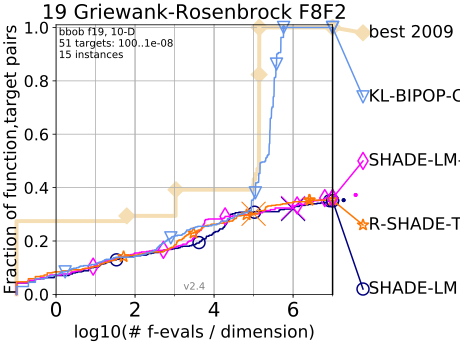
\includegraphics[width=0.2\textwidth]{pprldmany-single-functions/pprldmany_f019_10D}&
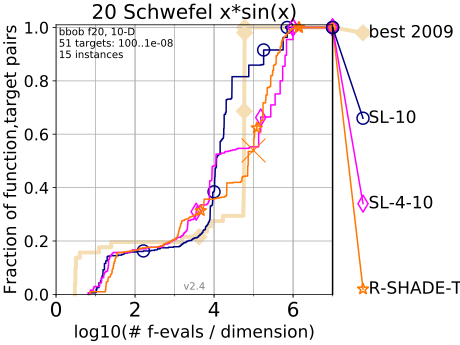
\includegraphics[width=0.2\textwidth]{pprldmany-single-functions/pprldmany_f020_10D}\\
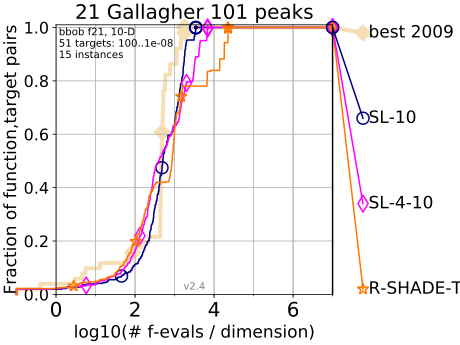
\includegraphics[width=0.2\textwidth]{pprldmany-single-functions/pprldmany_f021_10D}&
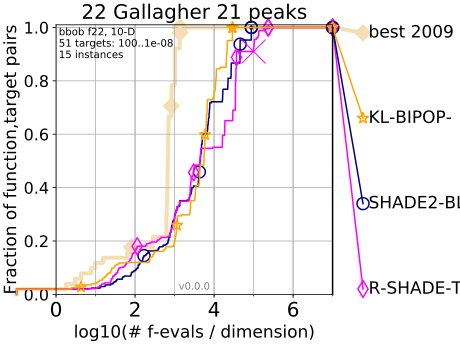
\includegraphics[width=0.2\textwidth]{pprldmany-single-functions/pprldmany_f022_10D}&
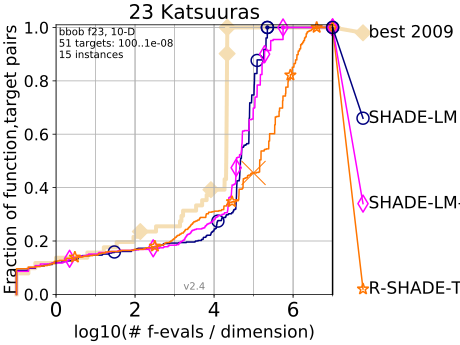
\includegraphics[width=0.2\textwidth]{pprldmany-single-functions/pprldmany_f023_10D}&
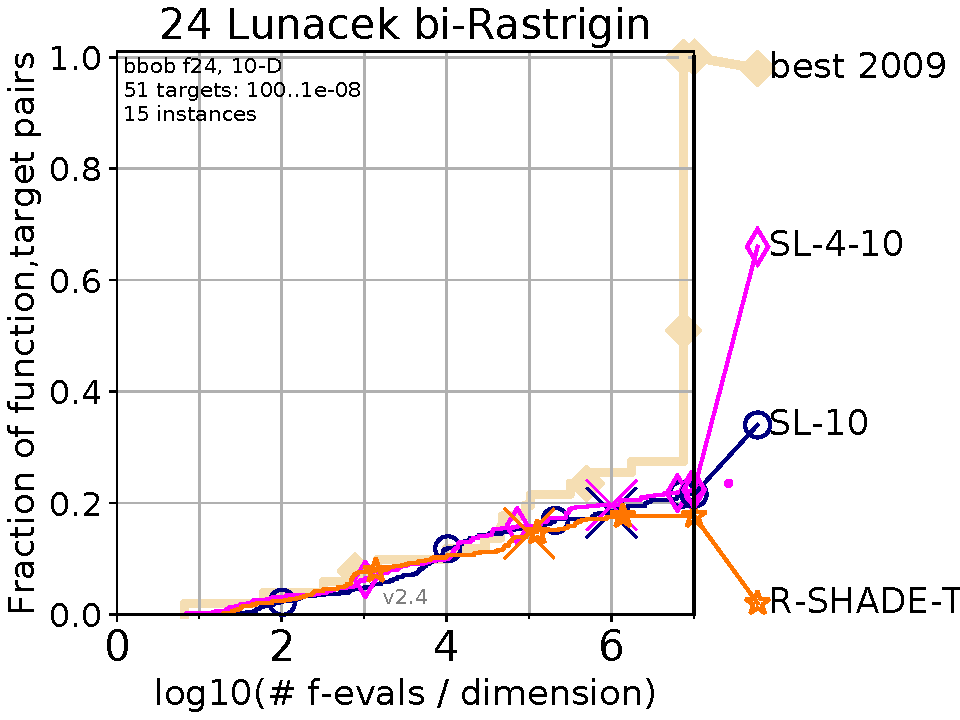
\includegraphics[width=0.2\textwidth]{pprldmany-single-functions/pprldmany_f024_10D}&
\includegraphics[width=0.2\textwidth]{pprldmany-single-functions/pprldmany_f025_10D}\\
\includegraphics[width=0.2\textwidth]{pprldmany-single-functions/pprldmany_f026_10D}&
\includegraphics[width=0.2\textwidth]{pprldmany-single-functions/pprldmany_f027_10D}&
\includegraphics[width=0.2\textwidth]{pprldmany-single-functions/pprldmany_f028_10D}&
\includegraphics[width=0.2\textwidth]{pprldmany-single-functions/pprldmany_f029_10D}&
\includegraphics[width=0.2\textwidth]{pprldmany-single-functions/pprldmany_f030_10D}\\
\includegraphics[width=0.2\textwidth]{pprldmany-single-functions/pprldmany_f031_10D}&
\includegraphics[width=0.2\textwidth]{pprldmany-single-functions/pprldmany_f032_10D}&
\includegraphics[width=0.2\textwidth]{pprldmany-single-functions/pprldmany_f033_10D}&
\includegraphics[width=0.2\textwidth]{pprldmany-single-functions/pprldmany_f034_10D}&
\includegraphics[width=0.2\textwidth]{pprldmany-single-functions/pprldmany_f035_10D}\\[-1.8ex]
\end{tabular}
 \caption{\label{fig:ECDFsingleOne}
	\bbobecdfcaptionsinglefunctionssingledim{10}
}
\end{figure*}

\begin{figure*}
\centering
\begin{tabular}{@{\hspace*{-0.00\textwidth}}l@{\hspace*{-0.00\textwidth}}l@{\hspace*{-0.00\textwidth}}l@{\hspace*{-0.00\textwidth}}l@{\hspace*{-0.00\textwidth}}l@{\hspace*{-0.00\textwidth}}}
\includegraphics[width=0.2\textwidth]{pprldmany-single-functions/pprldmany_f036_10D}&
\includegraphics[width=0.2\textwidth]{pprldmany-single-functions/pprldmany_f037_10D}&
\includegraphics[width=0.2\textwidth]{pprldmany-single-functions/pprldmany_f038_10D}&
\includegraphics[width=0.2\textwidth]{pprldmany-single-functions/pprldmany_f039_10D}&
\includegraphics[width=0.2\textwidth]{pprldmany-single-functions/pprldmany_f040_10D}\\
\includegraphics[width=0.2\textwidth]{pprldmany-single-functions/pprldmany_f041_10D}&
\includegraphics[width=0.2\textwidth]{pprldmany-single-functions/pprldmany_f042_10D}&
\includegraphics[width=0.2\textwidth]{pprldmany-single-functions/pprldmany_f043_10D}&
\includegraphics[width=0.2\textwidth]{pprldmany-single-functions/pprldmany_f044_10D}&
\includegraphics[width=0.2\textwidth]{pprldmany-single-functions/pprldmany_f045_10D}\\
\includegraphics[width=0.2\textwidth]{pprldmany-single-functions/pprldmany_f046_10D}&
\includegraphics[width=0.2\textwidth]{pprldmany-single-functions/pprldmany_f047_10D}&
\includegraphics[width=0.2\textwidth]{pprldmany-single-functions/pprldmany_f048_10D}&
\includegraphics[width=0.2\textwidth]{pprldmany-single-functions/pprldmany_f049_10D}&
\includegraphics[width=0.2\textwidth]{pprldmany-single-functions/pprldmany_f050_10D}\\
\includegraphics[width=0.2\textwidth]{pprldmany-single-functions/pprldmany_f051_10D}&
\includegraphics[width=0.2\textwidth]{pprldmany-single-functions/pprldmany_f052_10D}&
\includegraphics[width=0.2\textwidth]{pprldmany-single-functions/pprldmany_f053_10D}&
\includegraphics[width=0.2\textwidth]{pprldmany-single-functions/pprldmany_f054_10D}&
\includegraphics[width=0.2\textwidth]{pprldmany-single-functions/pprldmany_f055_10D}\\[-1.8ex]
\end{tabular}
 \caption{\label{fig:ECDFsingleTwo}
 Bootstrapped empirical cumulative distribution of the number of objective function evaluations divided by dimension (FEvals/DIM) as in Fig.~\ref{fig:ECDFsingleOne} but for functions $f_{36}$ to $f_{55}$ in 10-D.
}
\end{figure*}




%%%%%%%%%%%%%%%%%%%%%%%%%%%%%%%%%%%%%%%%%%%%%%%%%%%%%%%%%%%%%%%%%%%%%%%%%%%%%%%
%%%%%%%%%%%%%%%%%%%%%%%%%%%%%%%%%%%%%%%%%%%%%%%%%%%%%%%%%%%%%%%%%%%%%%%%%%%%%%%

% Empirical cumulative distribution functions (ECDFs) per function group (5-D)

%%%%%%%%%%%%%%%%%%%%%%%%%%%%%%%%%%%%%%%%%%%%%%%%%%%%%%%%%%%%%%%%%%%%%%%%%%%%%%%

\begin{figure*}
\begin{tabular}{@{\hspace*{-0.00\textwidth}}c@{\hspace*{-0.0\textwidth}}c@{\hspace*{-0.0\textwidth}}c@{\hspace*{-0.0\textwidth}}c}
separable-separable & separable-moderate & separable-ill-cond. & separable-multimodal\\
\includegraphics[width=0.24\textwidth]{pprldmany_05D_1-separable_1-separable} &
\includegraphics[width=0.24\textwidth]{pprldmany_05D_1-separable_2-moderate} &
\includegraphics[width=0.24\textwidth]{pprldmany_05D_1-separable_3-ill-conditioned} &
\includegraphics[width=0.24\textwidth]{pprldmany_05D_1-separable_4-multi-modal}\\
separable-weakstructure & moderate-moderate & moderate-ill-cond. & moderate-multimodal\\
\includegraphics[width=0.24\textwidth]{pprldmany_05D_1-separable_5-weakly-structured} &
\includegraphics[width=0.24\textwidth]{pprldmany_05D_2-moderate_2-moderate} &
\includegraphics[width=0.24\textwidth]{pprldmany_05D_2-moderate_3-ill-conditioned} &
\includegraphics[width=0.24\textwidth]{pprldmany_05D_2-moderate_4-multi-modal}\\
moderate-weakstructure & ill-cond.-ill-cond. & ill-cond.-multimodal & ill-cond.-weakstructure\\
\includegraphics[width=0.24\textwidth]{pprldmany_05D_2-moderate_5-weakly-structured} &
\includegraphics[width=0.24\textwidth]{pprldmany_05D_3-ill-conditioned_3-ill-conditioned} &
\includegraphics[width=0.24\textwidth]{pprldmany_05D_3-ill-conditioned_4-multi-modal} &
\includegraphics[width=0.24\textwidth]{pprldmany_05D_3-ill-conditioned_5-weakly-structured} \\
multimodal-multimodal & multimodal-weakstructure & weakstructure-weakstructure & all 55 functions\\
\includegraphics[width=0.24\textwidth]{pprldmany_05D_4-multi-modal_4-multi-modal} &
\includegraphics[width=0.24\textwidth]{pprldmany_05D_4-multi-modal_5-weakly-structured} &
\includegraphics[width=0.24\textwidth]{pprldmany_05D_5-weakly-structured_5-weakly-structured} &
\includegraphics[width=0.24\textwidth]{pprldmany_05D_noiselessall}
\vspace*{-0.5ex}
\end{tabular}
 \caption{\label{fig:ECDFsGroupsFive}
 \bbobECDFslegend{5}
 }
\end{figure*}

%%%%%%%%%%%%%%%%%%%%%%%%%%%%%%%%%%%%%%%%%%%%%%%%%%%%%%%%%%%%%%%%%%%%%%%%%%%%%%%
%%%%%%%%%%%%%%%%%%%%%%%%%%%%%%%%%%%%%%%%%%%%%%%%%%%%%%%%%%%%%%%%%%%%%%%%%%%%%%%

% Empirical cumulative distribution functions (ECDFs) per function group (20-D)

%%%%%%%%%%%%%%%%%%%%%%%%%%%%%%%%%%%%%%%%%%%%%%%%%%%%%%%%%%%%%%%%%%%%%%%%%%%%%%%

\begin{figure*}
\begin{tabular}{@{\hspace*{-0.00\textwidth}}c@{\hspace*{-0.0\textwidth}}c@{\hspace*{-0.0\textwidth}}c@{\hspace*{-0.0\textwidth}}c}
separable-separable & separable-moderate & separable-ill-cond. & separable-multimodal\\
\includegraphics[width=0.24\textwidth]{pprldmany_20D_1-separable_1-separable} &
\includegraphics[width=0.24\textwidth]{pprldmany_20D_1-separable_2-moderate} &
\includegraphics[width=0.24\textwidth]{pprldmany_20D_1-separable_3-ill-conditioned} &
\includegraphics[width=0.24\textwidth]{pprldmany_20D_1-separable_4-multi-modal}\\
separable-weakstructure & moderate-moderate & moderate-ill-cond. & moderate-multimodal\\
\includegraphics[width=0.24\textwidth]{pprldmany_20D_1-separable_5-weakly-structured} &
\includegraphics[width=0.24\textwidth]{pprldmany_20D_2-moderate_2-moderate} &
\includegraphics[width=0.24\textwidth]{pprldmany_20D_2-moderate_3-ill-conditioned} &
\includegraphics[width=0.24\textwidth]{pprldmany_20D_2-moderate_4-multi-modal}\\
moderate-weakstructure & ill-cond.-ill-cond. & ill-cond.-multimodal & ill-cond.-weakstructure\\
\includegraphics[width=0.24\textwidth]{pprldmany_20D_2-moderate_5-weakly-structured} &
\includegraphics[width=0.24\textwidth]{pprldmany_20D_3-ill-conditioned_3-ill-conditioned} &
\includegraphics[width=0.24\textwidth]{pprldmany_20D_3-ill-conditioned_4-multi-modal} &
\includegraphics[width=0.24\textwidth]{pprldmany_20D_3-ill-conditioned_5-weakly-structured} \\
multimodal-multimodal & multimodal-weakstructure & weakstructure-weakstructure & all 55 functions\\
\includegraphics[width=0.24\textwidth]{pprldmany_20D_4-multi-modal_4-multi-modal} &
\includegraphics[width=0.24\textwidth]{pprldmany_20D_4-multi-modal_5-weakly-structured} &
\includegraphics[width=0.24\textwidth]{pprldmany_20D_5-weakly-structured_5-weakly-structured} &
\includegraphics[width=0.24\textwidth]{pprldmany_20D_noiselessall}
\vspace*{-0.5ex}
\end{tabular}
 \caption{\label{fig:ECDFsGroupsTwenty}
 \bbobECDFslegend{20}
 }
\end{figure*}


\clearpage

%%%%%%%%%%%%%%%%%%%%%%%%%%%%%%%%%%%%%%%%%%%%%%%%%%%%%%%%%%%%%%%%%%%%%%%%%%%%%%%
%%%%%%%%%%%%%%%%%%%%%%%%%%%%%%%%%%%%%%%%%%%%%%%%%%%%%%%%%%%%%%%%%%%%%%%%%%%%%%%

% Expected runtime (ERT in number of function evaluations)
% for functions $f_1$--$f_{55}$ of the bbob-biobj suite for dimension 5.

%%%%%%%%%%%%%%%%%%%%%%%%%%%%%%%%%%%%%%%%%%%%%%%%%%%%%%%%%%%%%%%%%%%%%%%%%%%%%%%
{\normalsize \color{red}
\ifthenelse{\isundefined{\algorithmD}}{}{more than 3 algorithms: please split the tables below by hand until everything fits to the page limits}
}

\begin{table*}\tiny
\centering
\mbox{\begin{minipage}[t]{0.32\textwidth}\tiny
\centering

\pptablesheader

\input{\bbobdatapath\algsfolder pptables_f001_05D} 

\input{\bbobdatapath\algsfolder pptables_f002_05D}

\input{\bbobdatapath\algsfolder pptables_f003_05D}

\input{\bbobdatapath\algsfolder pptables_f004_05D}

\input{\bbobdatapath\algsfolder pptables_f005_05D}

\input{\bbobdatapath\algsfolder pptables_f006_05D}

\input{\bbobdatapath\algsfolder pptables_f007_05D}

\input{\bbobdatapath\algsfolder pptables_f008_05D}

\input{\bbobdatapath\algsfolder pptables_f009_05D}

\input{\bbobdatapath\algsfolder pptables_f010_05D}

\input{\bbobdatapath\algsfolder pptables_f011_05D}

\input{\bbobdatapath\algsfolder pptables_f012_05D}

\input{\bbobdatapath\algsfolder pptables_f013_05D}

\input{\bbobdatapath\algsfolder pptables_f014_05D}

\input{\bbobdatapath\algsfolder pptables_f015_05D}

\input{\bbobdatapath\algsfolder pptables_f016_05D}

\input{\bbobdatapath\algsfolder pptables_f017_05D}

\input{\bbobdatapath\algsfolder pptables_f018_05D}

\input{\bbobdatapath\algsfolder pptables_f019_05D}

\end{tabularx}

\end{minipage}
\hspace{0.002\textwidth}
\begin{minipage}[t]{0.32\textwidth}\tiny
\centering

\pptablesheader

\input{\bbobdatapath\algsfolder pptables_f020_05D}

\input{\bbobdatapath\algsfolder pptables_f021_05D}

\input{\bbobdatapath\algsfolder pptables_f022_05D}

\input{\bbobdatapath\algsfolder pptables_f023_05D}

\input{\bbobdatapath\algsfolder pptables_f024_05D}

\input{\bbobdatapath\algsfolder pptables_f025_05D}

\input{\bbobdatapath\algsfolder pptables_f026_05D}

\input{\bbobdatapath\algsfolder pptables_f027_05D}

\input{\bbobdatapath\algsfolder pptables_f028_05D}

\input{\bbobdatapath\algsfolder pptables_f029_05D}

\input{\bbobdatapath\algsfolder pptables_f030_05D}

\input{\bbobdatapath\algsfolder pptables_f031_05D}

\input{\bbobdatapath\algsfolder pptables_f032_05D}

\input{\bbobdatapath\algsfolder pptables_f033_05D}

\input{\bbobdatapath\algsfolder pptables_f034_05D}

\input{\bbobdatapath\algsfolder pptables_f035_05D}

\input{\bbobdatapath\algsfolder pptables_f036_05D}

\input{\bbobdatapath\algsfolder pptables_f037_05D}

\end{tabularx}

\end{minipage}

\hspace{0.002\textwidth}
\begin{minipage}[t]{0.32\textwidth}\tiny
\centering

\pptablesheader

\input{\bbobdatapath\algsfolder pptables_f038_05D}

\input{\bbobdatapath\algsfolder pptables_f039_05D}

\input{\bbobdatapath\algsfolder pptables_f040_05D}

\input{\bbobdatapath\algsfolder pptables_f041_05D}

\input{\bbobdatapath\algsfolder pptables_f042_05D}

\input{\bbobdatapath\algsfolder pptables_f043_05D}

\input{\bbobdatapath\algsfolder pptables_f044_05D}

\input{\bbobdatapath\algsfolder pptables_f045_05D}

\input{\bbobdatapath\algsfolder pptables_f046_05D}

\input{\bbobdatapath\algsfolder pptables_f047_05D}

\input{\bbobdatapath\algsfolder pptables_f048_05D}

\input{\bbobdatapath\algsfolder pptables_f049_05D}

\input{\bbobdatapath\algsfolder pptables_f050_05D}

\input{\bbobdatapath\algsfolder pptables_f051_05D}

\input{\bbobdatapath\algsfolder pptables_f052_05D}

\input{\bbobdatapath\algsfolder pptables_f053_05D}

\input{\bbobdatapath\algsfolder pptables_f054_05D}

\input{\bbobdatapath\algsfolder pptables_f055_05D}

\end{tabularx}

\end{minipage}}

 \caption{\label{tab:ERTs5}
 \bbobpptablesmanylegend{dimension $5$}
 }
\end{table*}
%sideways


%%%%%%%%%%%%%%%%%%%%%%%%%%%%%%%%%%%%%%%%%%%%%%%%%%%%%%%%%%%%%%%%%%%%%%%%%%%%%%%
%%%%%%%%%%%%%%%%%%%%%%%%%%%%%%%%%%%%%%%%%%%%%%%%%%%%%%%%%%%%%%%%%%%%%%%%%%%%%%%

% Expected runtime (ERT in number of function evaluations)
% for functions $f_1$--$f_{55}$ of the bbob-biobj suite for dimension 20.

%%%%%%%%%%%%%%%%%%%%%%%%%%%%%%%%%%%%%%%%%%%%%%%%%%%%%%%%%%%%%%%%%%%%%%%%%%%%%%%
\begin{table*}\tiny
\centering
\mbox{\begin{minipage}[t]{0.32\textwidth}\tiny
\centering

\pptablesheader

\input{\bbobdatapath\algsfolder pptables_f001_20D} 

\input{\bbobdatapath\algsfolder pptables_f002_20D}

\input{\bbobdatapath\algsfolder pptables_f003_20D}

\input{\bbobdatapath\algsfolder pptables_f004_20D}

\input{\bbobdatapath\algsfolder pptables_f005_20D}

\input{\bbobdatapath\algsfolder pptables_f006_20D}

\input{\bbobdatapath\algsfolder pptables_f007_20D}

\input{\bbobdatapath\algsfolder pptables_f008_20D}

\input{\bbobdatapath\algsfolder pptables_f009_20D}

\input{\bbobdatapath\algsfolder pptables_f010_20D}

\input{\bbobdatapath\algsfolder pptables_f011_20D}

\input{\bbobdatapath\algsfolder pptables_f012_20D}

\input{\bbobdatapath\algsfolder pptables_f013_20D}

\input{\bbobdatapath\algsfolder pptables_f014_20D}

\input{\bbobdatapath\algsfolder pptables_f015_20D}

\input{\bbobdatapath\algsfolder pptables_f016_20D}

\input{\bbobdatapath\algsfolder pptables_f017_20D}

\input{\bbobdatapath\algsfolder pptables_f018_20D}

\input{\bbobdatapath\algsfolder pptables_f019_20D}

\end{tabularx}

\end{minipage}
\hspace{0.002\textwidth}
\begin{minipage}[t]{0.32\textwidth}\tiny
\centering

\pptablesheader

\input{\bbobdatapath\algsfolder pptables_f020_20D}

\input{\bbobdatapath\algsfolder pptables_f021_20D}

\input{\bbobdatapath\algsfolder pptables_f022_20D}

\input{\bbobdatapath\algsfolder pptables_f023_20D}

\input{\bbobdatapath\algsfolder pptables_f024_20D}

\input{\bbobdatapath\algsfolder pptables_f025_20D}

\input{\bbobdatapath\algsfolder pptables_f026_20D}

\input{\bbobdatapath\algsfolder pptables_f027_20D}

\input{\bbobdatapath\algsfolder pptables_f028_20D}

\input{\bbobdatapath\algsfolder pptables_f029_20D}

\input{\bbobdatapath\algsfolder pptables_f030_20D}

\input{\bbobdatapath\algsfolder pptables_f031_20D}

\input{\bbobdatapath\algsfolder pptables_f032_20D}

\input{\bbobdatapath\algsfolder pptables_f033_20D}

\input{\bbobdatapath\algsfolder pptables_f034_20D}

\input{\bbobdatapath\algsfolder pptables_f035_20D}

\input{\bbobdatapath\algsfolder pptables_f036_20D}

\input{\bbobdatapath\algsfolder pptables_f037_20D}

\end{tabularx}

\end{minipage}

\hspace{0.002\textwidth}
\begin{minipage}[t]{0.32\textwidth}\tiny
\centering

\pptablesheader

\input{\bbobdatapath\algsfolder pptables_f038_20D}

\input{\bbobdatapath\algsfolder pptables_f039_20D}

\input{\bbobdatapath\algsfolder pptables_f040_20D}

\input{\bbobdatapath\algsfolder pptables_f041_20D}

\input{\bbobdatapath\algsfolder pptables_f042_20D}

\input{\bbobdatapath\algsfolder pptables_f043_20D}

\input{\bbobdatapath\algsfolder pptables_f044_20D}

\input{\bbobdatapath\algsfolder pptables_f045_20D}

\input{\bbobdatapath\algsfolder pptables_f046_20D}

\input{\bbobdatapath\algsfolder pptables_f047_20D}

\input{\bbobdatapath\algsfolder pptables_f048_20D}

\input{\bbobdatapath\algsfolder pptables_f049_20D}

\input{\bbobdatapath\algsfolder pptables_f050_20D}

\input{\bbobdatapath\algsfolder pptables_f051_20D}

\input{\bbobdatapath\algsfolder pptables_f052_20D}

\input{\bbobdatapath\algsfolder pptables_f053_20D}

\input{\bbobdatapath\algsfolder pptables_f054_20D}

\input{\bbobdatapath\algsfolder pptables_f055_20D}

\end{tabularx}

\end{minipage}}

 \caption{\label{tab:ERTs20}
 \bbobpptablesmanylegend{dimension $20$}
 }
\end{table*}



%%%%%%%%%%%%%%%%%%%%%%%%%%%%%%%%%%%%%%%%%%%%%%%%%%%%%%%%%%%%%%%%%%%%%%%%%%%%%%%
%%%%%%%%%%%%%%%%%%%%%%%%%%%%%%%%%%%%%%%%%%%%%%%%%%%%%%%%%%%%%%%%%%%%%%%%%%%%%%%

\bibliographystyle{ACM-Reference-Format}
\bibliography{bbob}  % bbob.bib is the name of the Bibliography in this case

%%%%%%%%%%%%%%%%%%%%%%%%%%%%%%%%%%%%%%%%%%%%%%%%%%%%%%%%%%%%%%%%%%%%%%%%%%%%%%%%%%%%%%%%%%%

\clearpage % otherwise the last figure might be missing
\appendix

The following pages present additional results that do not fit into the actual paper due to the page limit.


%%%%%%%%%%%%%%%%%%%%%%%%%%%%%%%%%%%%%%%%%%%%%%%%%%%%%%%%%%%%%%%%%%%%%%%%%%%%%%%
%%%%%%%%%%%%%%%%%%%%%%%%%%%%%%%%%%%%%%%%%%%%%%%%%%%%%%%%%%%%%%%%%%%%%%%%%%%%%%%

% Scaling of ERT with dimension

%%%%%%%%%%%%%%%%%%%%%%%%%%%%%%%%%%%%%%%%%%%%%%%%%%%%%%%%%%%%%%%%%%%%%%%%%%%%%%%
\begin{figure*}
\begin{tabular}{@{\hspace*{-0.0\textwidth}}l@{\hspace*{-0.0\textwidth}}l@{\hspace*{-0.0\textwidth}}l@{\hspace*{-0.0\textwidth}}l@{\hspace*{-0.0\textwidth}}l@{\hspace*{-0.0\textwidth}}}
\includegraphics[width=0.2\textwidth]{ppfigs_f001}&
\includegraphics[width=0.2\textwidth]{ppfigs_f002}&
\includegraphics[width=0.2\textwidth]{ppfigs_f003}&
\includegraphics[width=0.2\textwidth]{ppfigs_f004}&
\includegraphics[width=0.2\textwidth]{ppfigs_f005}\\
\includegraphics[width=0.2\textwidth]{ppfigs_f006}&
\includegraphics[width=0.2\textwidth]{ppfigs_f007}&
\includegraphics[width=0.2\textwidth]{ppfigs_f008}&
\includegraphics[width=0.2\textwidth]{ppfigs_f009}&
\includegraphics[width=0.2\textwidth]{ppfigs_f010}\\
\includegraphics[width=0.2\textwidth]{ppfigs_f011}&
\includegraphics[width=0.2\textwidth]{ppfigs_f012}&
\includegraphics[width=0.2\textwidth]{ppfigs_f013}&
\includegraphics[width=0.2\textwidth]{ppfigs_f014}&
\includegraphics[width=0.2\textwidth]{ppfigs_f015}\\
\includegraphics[width=0.2\textwidth]{ppfigs_f016}&
\includegraphics[width=0.2\textwidth]{ppfigs_f017}&
\includegraphics[width=0.2\textwidth]{ppfigs_f018}&
\includegraphics[width=0.2\textwidth]{ppfigs_f019}&
\includegraphics[width=0.2\textwidth]{ppfigs_f020}\\
\includegraphics[width=0.2\textwidth]{ppfigs_f021}&
\includegraphics[width=0.2\textwidth]{ppfigs_f022}&
\includegraphics[width=0.2\textwidth]{ppfigs_f023}&
\includegraphics[width=0.2\textwidth]{ppfigs_f024}&
\includegraphics[width=0.2\textwidth]{ppfigs_f025}\\
\includegraphics[width=0.2\textwidth]{ppfigs_f026}&
\includegraphics[width=0.2\textwidth]{ppfigs_f027}&
\includegraphics[width=0.2\textwidth]{ppfigs_f028}&
\includegraphics[width=0.2\textwidth]{ppfigs_f029}&
\includegraphics[width=0.2\textwidth]{ppfigs_f030}
\end{tabular}
\vspace{-3ex}
\caption[Expected running time divided by dimension
         versus dimension]{
         \label{fig:scaling1}
         \bbobppfigslegend{$f_1$ and $f_{30}$}
}
\end{figure*}

\begin{figure*}
\begin{tabular}{@{\hspace*{-0.0\textwidth}}l@{\hspace*{-0.0\textwidth}}l@{\hspace*{-0.0\textwidth}}l@{\hspace*{-0.0\textwidth}}l@{\hspace*{-0.0\textwidth}}l@{\hspace*{-0.0\textwidth}}}
\includegraphics[width=0.2\textwidth]{ppfigs_f031}&
\includegraphics[width=0.2\textwidth]{ppfigs_f032}&
\includegraphics[width=0.2\textwidth]{ppfigs_f033}&
\includegraphics[width=0.2\textwidth]{ppfigs_f034}&
\includegraphics[width=0.2\textwidth]{ppfigs_f035}\\
\includegraphics[width=0.2\textwidth]{ppfigs_f036}&
\includegraphics[width=0.2\textwidth]{ppfigs_f037}&
\includegraphics[width=0.2\textwidth]{ppfigs_f038}&
\includegraphics[width=0.2\textwidth]{ppfigs_f039}&
\includegraphics[width=0.2\textwidth]{ppfigs_f040}\\
\includegraphics[width=0.2\textwidth]{ppfigs_f041}&
\includegraphics[width=0.2\textwidth]{ppfigs_f042}&
\includegraphics[width=0.2\textwidth]{ppfigs_f043}&
\includegraphics[width=0.2\textwidth]{ppfigs_f044}&
\includegraphics[width=0.2\textwidth]{ppfigs_f045}\\
\includegraphics[width=0.2\textwidth]{ppfigs_f046}&
\includegraphics[width=0.2\textwidth]{ppfigs_f047}&
\includegraphics[width=0.2\textwidth]{ppfigs_f048}&
\includegraphics[width=0.2\textwidth]{ppfigs_f049}&
\includegraphics[width=0.2\textwidth]{ppfigs_f050}\\
\includegraphics[width=0.2\textwidth]{ppfigs_f051}&
\includegraphics[width=0.2\textwidth]{ppfigs_f052}&
\includegraphics[width=0.2\textwidth]{ppfigs_f053}&
\includegraphics[width=0.2\textwidth]{ppfigs_f054}&
\includegraphics[width=0.2\textwidth]{ppfigs_f055}
\end{tabular}
\vspace{-3ex}
\caption[Expected running time divided by dimension
         versus dimension]{
         \label{fig:scaling2}
         \bbobppfigslegend{$f_{31}$ and $f_{55}$}
}
\end{figure*}

\IfFileExists{\bbobdatapath\algsfolder ppfig2_f001.pdf}{}{\end{document}}

%%%%%%%%%%%%%%%%%%%%%%%%%%%%%%%%%%%%%%%%%%%%%%%%%%%%%%%%%%%%%%%%%%%%%%%%%%%%%%%
%%%%%%%%%%%%%%%%%%%%%%%%%%%%%%%%%%%%%%%%%%%%%%%%%%%%%%%%%%%%%%%%%%%%%%%%%%%%%%%
% Scatter plots per function.
%%%%%%%%%%%%%%%%%%%%%%%%%%%%%%%%%%%%%%%%%%%%%%%%%%%%%%%%%%%%%%%%%%%%%%%%%%%%%%%
%%%%%%%%%%%%%%%%%%%%%%%%%%%%%%%%%%%%%%%%%%%%%%%%%%%%%%%%%%%%%%%%%%%%%%%%%%%%%%%
\newcommand{\rot}[2][2.5]{
  \hspace*{-3.5\baselineskip}%
  \begin{rotate}{90}\hspace{#1em}#2
  \end{rotate}}
%%%%%%%%%%%%%%%%%%%%%%%%%%%%%%%%%%%%%%%%%%%%%%%%%%%%%%%%%%%%%%%%%%%%%%%%%%%%%%%
%%%%%%%%%%%%%%%%%%%%%%%%%%%%%%%%%%%%%%%%%%%%%%%%%%%%%%%%%%%%%%%%%%%%%%%%%%%%%%%
\begin{figure*}
\centering
\begin{tabular}{*{5}{@{}c@{}}}
    \includegraphics[width=0.20\textwidth]{ppscatter_f001}&
    \includegraphics[width=0.20\textwidth]{ppscatter_f002}&
    \includegraphics[width=0.20\textwidth]{ppscatter_f003}& 
    \includegraphics[width=0.20\textwidth]{ppscatter_f004}&
    \includegraphics[width=0.20\textwidth]{ppscatter_f005}\\
    \includegraphics[width=0.20\textwidth]{ppscatter_f006}&
    \includegraphics[width=0.20\textwidth]{ppscatter_f007}&
    \includegraphics[width=0.20\textwidth]{ppscatter_f008}&
    \includegraphics[width=0.20\textwidth]{ppscatter_f009}&
    \includegraphics[width=0.20\textwidth]{ppscatter_f010}\\
    \includegraphics[width=0.20\textwidth]{ppscatter_f011}&
    \includegraphics[width=0.20\textwidth]{ppscatter_f012}&
    \includegraphics[width=0.20\textwidth]{ppscatter_f013}&
    \includegraphics[width=0.20\textwidth]{ppscatter_f014}&
    \includegraphics[width=0.20\textwidth]{ppscatter_f015}\\
    \includegraphics[width=0.20\textwidth]{ppscatter_f016}&
    \includegraphics[width=0.20\textwidth]{ppscatter_f017}&
    \includegraphics[width=0.20\textwidth]{ppscatter_f018}&
    \includegraphics[width=0.20\textwidth]{ppscatter_f019}&
    \includegraphics[width=0.20\textwidth]{ppscatter_f020}\\
    \includegraphics[width=0.20\textwidth]{ppscatter_f021}&
    \includegraphics[width=0.20\textwidth]{ppscatter_f022}&
    \includegraphics[width=0.20\textwidth]{ppscatter_f023}&
    \includegraphics[width=0.20\textwidth]{ppscatter_f024}&
		\includegraphics[width=0.20\textwidth]{ppscatter_f025}\\
		\includegraphics[width=0.20\textwidth]{ppscatter_f026}&
    \includegraphics[width=0.20\textwidth]{ppscatter_f027}&
    \includegraphics[width=0.20\textwidth]{ppscatter_f028}&
    \includegraphics[width=0.20\textwidth]{ppscatter_f029}&
		\includegraphics[width=0.20\textwidth]{ppscatter_f030}
\end{tabular}
\caption{\label{fig:scatterplots}
\bbobppscatterlegend{$f_1$--$f_{30}$}
}
\end{figure*}

\begin{figure*}
\centering
\begin{tabular}{*{5}{@{}c@{}}}
    \includegraphics[width=0.20\textwidth]{ppscatter_f031}&
    \includegraphics[width=0.20\textwidth]{ppscatter_f032}&
    \includegraphics[width=0.20\textwidth]{ppscatter_f033}& 
    \includegraphics[width=0.20\textwidth]{ppscatter_f034}&
    \includegraphics[width=0.20\textwidth]{ppscatter_f035}\\
    \includegraphics[width=0.20\textwidth]{ppscatter_f036}&
    \includegraphics[width=0.20\textwidth]{ppscatter_f037}&
    \includegraphics[width=0.20\textwidth]{ppscatter_f038}&
    \includegraphics[width=0.20\textwidth]{ppscatter_f039}&
    \includegraphics[width=0.20\textwidth]{ppscatter_f040}\\
    \includegraphics[width=0.20\textwidth]{ppscatter_f041}&
    \includegraphics[width=0.20\textwidth]{ppscatter_f042}&
    \includegraphics[width=0.20\textwidth]{ppscatter_f043}&
    \includegraphics[width=0.20\textwidth]{ppscatter_f044}&
    \includegraphics[width=0.20\textwidth]{ppscatter_f045}\\
    \includegraphics[width=0.20\textwidth]{ppscatter_f046}&
    \includegraphics[width=0.20\textwidth]{ppscatter_f047}&
    \includegraphics[width=0.20\textwidth]{ppscatter_f048}&
    \includegraphics[width=0.20\textwidth]{ppscatter_f049}&
    \includegraphics[width=0.20\textwidth]{ppscatter_f050}\\
    \includegraphics[width=0.20\textwidth]{ppscatter_f051}&
    \includegraphics[width=0.20\textwidth]{ppscatter_f052}&
    \includegraphics[width=0.20\textwidth]{ppscatter_f053}&
    \includegraphics[width=0.20\textwidth]{ppscatter_f054}&
		\includegraphics[width=0.20\textwidth]{ppscatter_f055}
\end{tabular}
\caption{\label{fig:scatterplots}
\bbobppscatterlegend{$f_{31}$--$f_{55}$}
}
\end{figure*}


\end{document}



